\documentclass{dhbenelux}
\usepackage{amsmath}

\usepackage{booktabs} % for toprule, midrule, bottomrule in tables
\usepackage{authblk} % for multiple authors and affiliations
\usepackage{graphicx} % to inlcude graphics with \includegraphics

\author[1]{Federico Porcelli}
\author[2]{Rocky Kamen-Rubio}

\affil[1]{Freie Universitaet Berlin}

\title{Nuclear Magnetic Resonance}

\begin{document}

\maketitle

\section{Introduction}

\subsection{What is NMR?}

NMR = Nuclear Magnetic Resonance is phenomenon in which atomic nuclei interact with electromagnetic radiation due to their magnetic dipole. It has applications in material measurement, especially in medecine (MRI machines).


\subsection{Why nuclei have spin? Which samples will you measure and what exactly will give you the signal in the experiment?}

From quantum mechanical theory, recall that protons and neutrons have a property called "spin", which behaves like angular momentum. So also the nuclei have spin, namely a spin system composed of protons and neutrons, and the interaction strength of the EM radiation depends on spin (i.e. quantum state) and type of nucleus (element). As a consequence, nuclei with L = 0 (where L is the angular momentum quantum number of the nucleus) do not interact, and are thus "invisible", e.g. $^{12}\text{C}$, $^{16}\text{O}$. % though the underlying mechanism is beyond the scope of this experiment and still poorly understood.

\begin{figure}[h!]
  \centering
  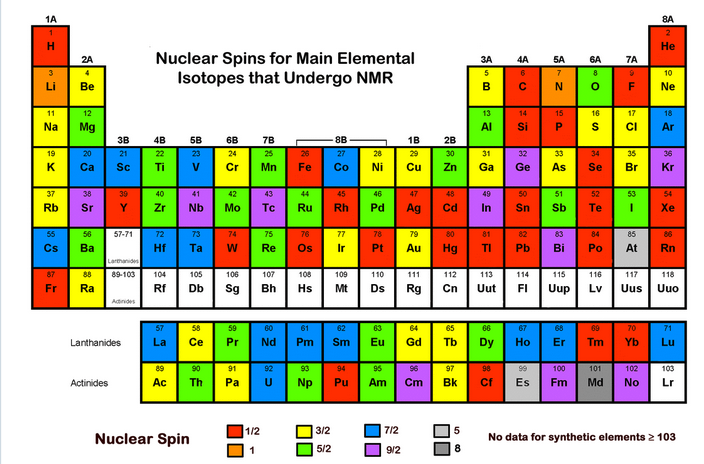
\includegraphics[width=0.7\textwidth]{element_spin.png}
  \caption{Table illustrating nuclear spins for different elements \cite{mri_questions_nuclear_spin}}
  \label{fig:example}
\end{figure}


\subsection{How do you understand "spin"? What is the gyromagnetic ratio of a proton?}

The gyromagnetic ratio $(\gamma)$ is defined as the ratio of the magnetic moment to the angular momentum.

\[\gamma = \frac{\mu}{L}\]

More intuitively, this can be thought of as "how strongly a given configuration interacts with a B-field", or "how much magnetic moment you get per angular momentum". The gyromagnetic ratio of a proton $\gamma_{proton} \approx 2.68 s^{-1}T^{-1}$ (there is some theory around why this is the value but it is not relevant right now). Recall as well that the energy of a magnetic moment $\mu$ in a magnetic field $B$ is $-\mu B$

\subsection{What happens to a nuclear spin in a magnetic field (Zeeman splitting, Larmor precession, Larmor frequency)}

A magnetic field will cause the particles to align their magnetic dipoles with the field. They can align with the field, in what is called the $\alpha$ state, or antiparellel to it, in what we call the $\beta$ state. The difference between these two energy states will be

\[\Delta E = \frac{\gamma \hbar B_0}{2\pi} \]

Note that this split is proportional to the applied magnetic field. When we consider that spin quantum number $m_I \in {-I, ..., I}$, we get

\[E = E_0 - \frac{\hbar \gamma B_0 m_I}{2\pi}\]



% This will cause some energy levels to split (Zeeman splitting). These energies are given by

% \[ E_m = -m\gamma \hbar B_0\]

% Where m is the magnetic quantum number, given by $m = -I, -I - 1, ..., I-1, I$ where I is the spin of the nucleus.

Larmor procession is procession that will occur by the magnetic moments around the applied B-field. This behaves as expected with a classical gyroscope, we call its frequency the \textbf{Larmor frequency} and it is

\[ \omega_L = \gamma B_0\]

(do we need to show the derivation?)

\subsection{ Ensemble of spins. Populations of the spin levels. Macroscopic magnetization vector. Dynamics of the magnetization vector in the external magnetic field.}

Without an external magnetic field, the sum of all magnetic moments cancels, and thus no population difference between two spin states can exist (equal distribution of spin up-spin down particles). However, when we introduce an external magnetic field, a difference in the population of two spin states occurs, which results in a net magnetization parallel to the applied field.

The energy difference of states leads to a difference in population

\[\frac{N_{upper}}{N_{lower}} = exp({\frac{-\Delta E}{kT}}) = exp({\frac{-h \nu}{kT}}) = exp({\frac{\gamma h B_0}{2\pi kT}})\]

%Particles in spin pairs will have no contribution to spin. We will call $N$ the number of non-paired particles that are "participating" in our spin ensemble. The distribution of particles in states will follow the Boltzman distribution


The strength of the signal observed will be

\[S(t) = N_{tot}Psin(\theta)\gamma B cos(\omega t)\]

Where P, the polarization is defined as

\[P = \frac{N_{\uparrow} - N_{\downarrow}}{N_{\uparrow} + N_{\downarrow}} = \frac{\gamma \hbar B_0}{2kT}\]

Is it necessary to show the derivation here?

At $T= 300K$ and $B_0 = 1T$ for protons we have $P = .0000034$ \cite{pirl_youtube_mri}
\\\

More generally a sample in thermal equilibrium will have

\[S = \frac{N_{tot}\gamma^3\hbar^2B_0^2}{4kT}\]


We define the Boltzmann Magnetization $M_0$ as

\[M_0 = \sum \vec{\mu} \cdot density \cdot P = \frac{N\gamma^2\hbar^2B_0}{4kT} = \chai_0 B_0\]

\subsection { Magnetic resonance: What is resonating?}

If we apply a B field to a nuclear with magnetic moment that is not already aligned with the field, it will experience Larmor precession. This precession will emit a specific frequency depending on the gyromagnetic ratio and magnitude of the applied B-field, that we can measure. If we apply this perpendicular B-field at the Larmor frequency, we can induce resonance.
Thus the spinning nuclei will precess with a frequency proportional to the applied magnetic field, i.e.:
\[\nu_L = \frac{\gamma B_0}{2\pi}\]

\subsection {Rotating frame vs. laboratory frame. Dynamics of the magnetization vector: Blochs equations of motion.}

After the nuclei have been pulsed, their magnetic moments proceed in a corkscrew pattern as they process and reconverge around the baseline magnetic field $B_0$. This is easier to describe mathematically in a rotating reference frame centered on a nucleus with rotation rate equal to the Larmor frequency. Here we can just look at the behavior of the components of the nucleus magnetic moment in the $B0$ and $B_1$ directions, as one decays and the other approaches $\mu$

\subsection { π/2 pulse. FID (free induction decay) with no relaxation processes. How do we detect an FID from an ensemble of magnetic nuclei? Sketch a setup.}

FID can be observed from the procession of the ensemble of magnetic moments around the applied constant magnetic field $B_0$ when an orthogonal pulse is applied close to the Larmor frequency.

\begin{figure}[h!]
  \centering
  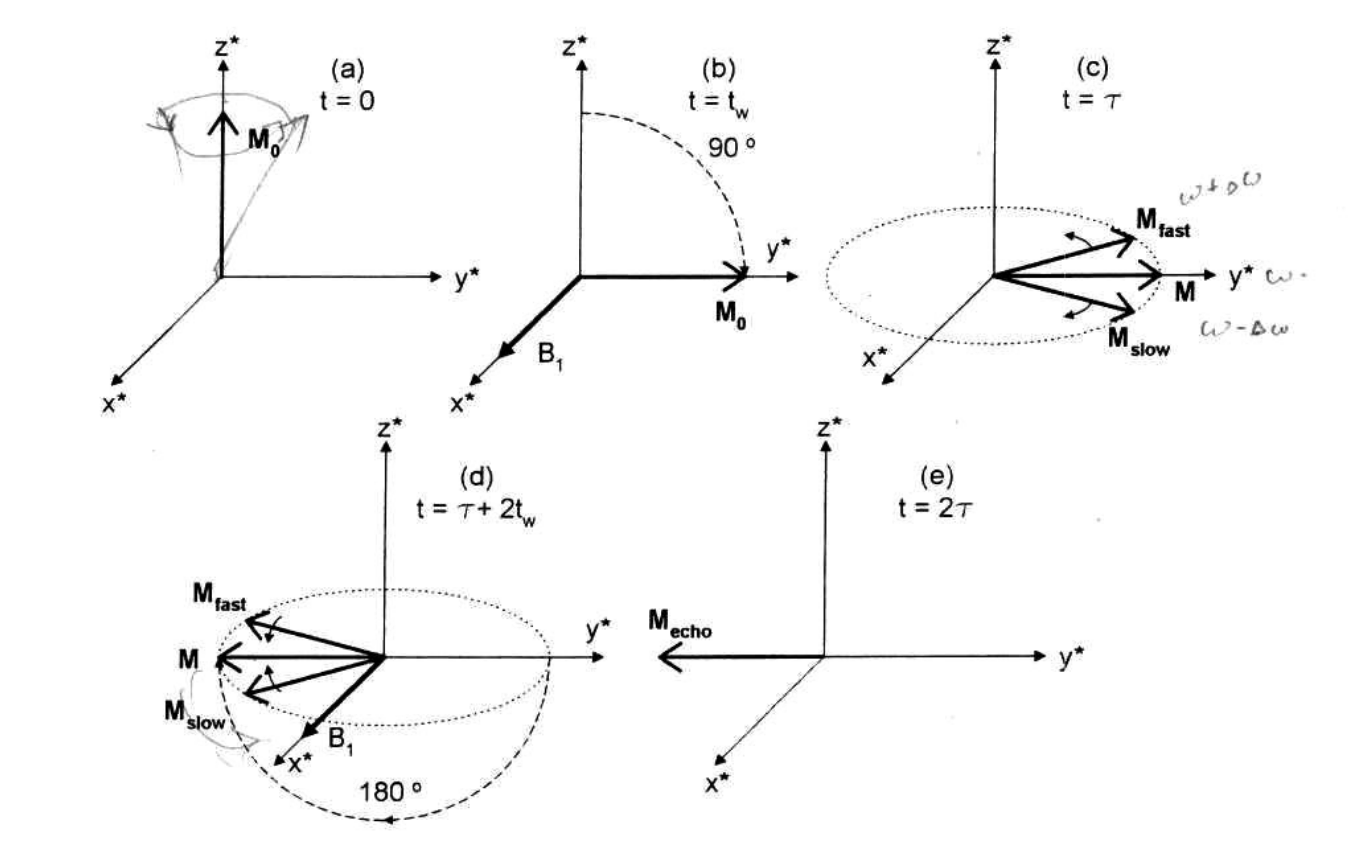
\includegraphics[width=0.7\textwidth]{FID.png}
  \caption{Schematic illustrating each stage of FID \cite{pulsed_spectrometer_manual}}
  \label{fig:example}
\end{figure}



\subsection {Relaxation times. T1 vs. T2 vs. T2*. You should know the differences between them.}

Since we need to observe many nuclei in aggregate to have a measurable effect, the nuclei need to all be precessing in phase. They will randomly become out of phase over time after the aligning pulse has been applied due to each other's magnetic fields, and other non-uniform magnetic fields. This leads to the overall signal strength decaying according to the Free Induction Decay (FID).

\[S(t) = Acos(\omega t)e^{-t/T_2}\]

The nuclei will also converge over time back to being in line with the base magnetic field, by the following magnitization

\[M(t) = M_0(1-e^{-t/T_1})\]

Where $T_1$ represents the rate at which the nuclei return to allignment with the base magnetid field.


\subsection{Bloch equations}

The Bloch equations refer to the following electrostatic relations. Definitionally, the torque is the cross product of the magnetic moment with the applied B-field.

\[\vec{T} = \vec{M} \times \vec{B}\]

We also can describe the torque as

\[ \vec{T} = \frac{\partial{\vec{J}}}{\partial{\vec{t}}}\]

And writing the magnetic moment as the sum of parts, and substituting the gyromagnetic ratio

\[\vec{M} = \sum_i\mu_i = \sum_i\gamma \vec{J_i}\]

\[ \frac{\partial \vec{M}}{\partial t} = \gamma \frac{\partial}{\partial t}\vec{J} = \gamma \vec{T} = \gamma(\vec{M} \times \vec{B})\]

When we only have the $B_0$ field applied along the z-axis, we get the following set of coupled differential equations

\[ \frac{\partial}{\partial t} M_x(t) = \gamma M_y B_0 - M_x/T_2\]
\[ \frac{\partial}{\partial t} M_y(t) = -\gamma M_x B_0 - M_y/T_2\]
\[ \frac{\partial}{\partial t} M_z(t) = -(M_z - M_0)/T_1\]

Which have solutions

\[M_x(t) = [M_x(0)cos(\omega t) - M_y(0)sin(\omega t)]e^{-t/T_2}\]
\[M_y(t) = [M_x(0)sin(\omega t) - M_y(0)cos(\omega t)]e^{-t/T_2}\]
\[M_z(t) = M_{eq} + [M_z(0) - M_{eq}]e^{-t/T_1}\]




\subsection{Spin echo. Pulse sequences.}

Suppose we give a pulse $B_1$. Subsequently we apply another pulse with the same magnitude and opposite direction of $B_1$ at time $\tau$ after the first pulse. All the magnetic moments became out of phase due to inhomogeneities in the constant magnetic field. Assuming these inhomogeneities are constant, this second pulse will reverse the trajectory of all these moments, and will reconverge at their initial configuration from the first pulse after another interval of $\tau$.

\subsection{T2 and T2* measurements}

T2* is the decay rate of the signal when we take into account imperfections in the applied fields. A proton has $\gamma = 42.6 MHz/T$, so if we change $B= 1T$ to $B = 1.000001T$ (an error of order $10^{-6}$), this can produce a change of

\[\Delta \omega = \gamma \Delta B = 267.5 rad/s\]

Assuming our decay is still perfectly exponential with the inhomogeneity, and the effect of the inhomogeneity can be represented as a single exponential term, we have

\[S(t)=S_0e^{-t/T_2^*} = S_0e^{-t/T_2}e^{-\gamma \Delta B t}\]

\[\frac{1}{T_2^*} = \frac{1}{T_2} + \gamma \Delta B\]

(do we need to talk about wy this assumption is valid? The Lorenztian distribution?)

Any magnetic field will have some inhomogeneity, which will put a lower bound on our error no matter how high we raise $T_2$

\subsection{T1 (spin-lattice relaxation time) measurement.}

Spin lattice relaxation time is our T1 relaxation time, spin-spin is our T2 relaxation time.

The Carr-Purcell method involves applying a $90^o$ pulse, following by a series of $180^o$ pulses separated by some time $\tau$, which is short compared to either of the relaxation times. This causes the moments to become coherent again after the diffuse following the first pulse. Repeating this process allows us to see this process multiple times. The Meiboom-Gill enhancement applies a $90^o$ shift at each successive pulse, which eliminates some of the error accumulation from the Carr-Pucell method


\section{ Experimental Setup}

We will use a light mineral oil and several concentrations of $CuSO_4$ samples and observe it with a TeachSpin PS2-A pulse spectrometer.
The sample is positioned in a coil, which is inside the $B_0$ field. This coil firstly acts as an transmitter, i.e. it supplies a RF wave that changes the net magnetization of the sample. Then, after the signal has been applied, the same coil acts as a "receiver" (pickup coil), and records the precession of the B field in the x-y plane.

The PS2-A Synthesizer module is used to produce the oscillating RF signal that "tips" the spins, altering the net magnetization of the sample. Then the Pulse Programmer module is used to determine the duration and number of the RF pulses. Finally, the Receiver takes care of the amplification of the RF signal going into the coil, and directs the incoming RF resulting from the sample to the oscilloscope.
\begin{figure}[h!]
  \centering
  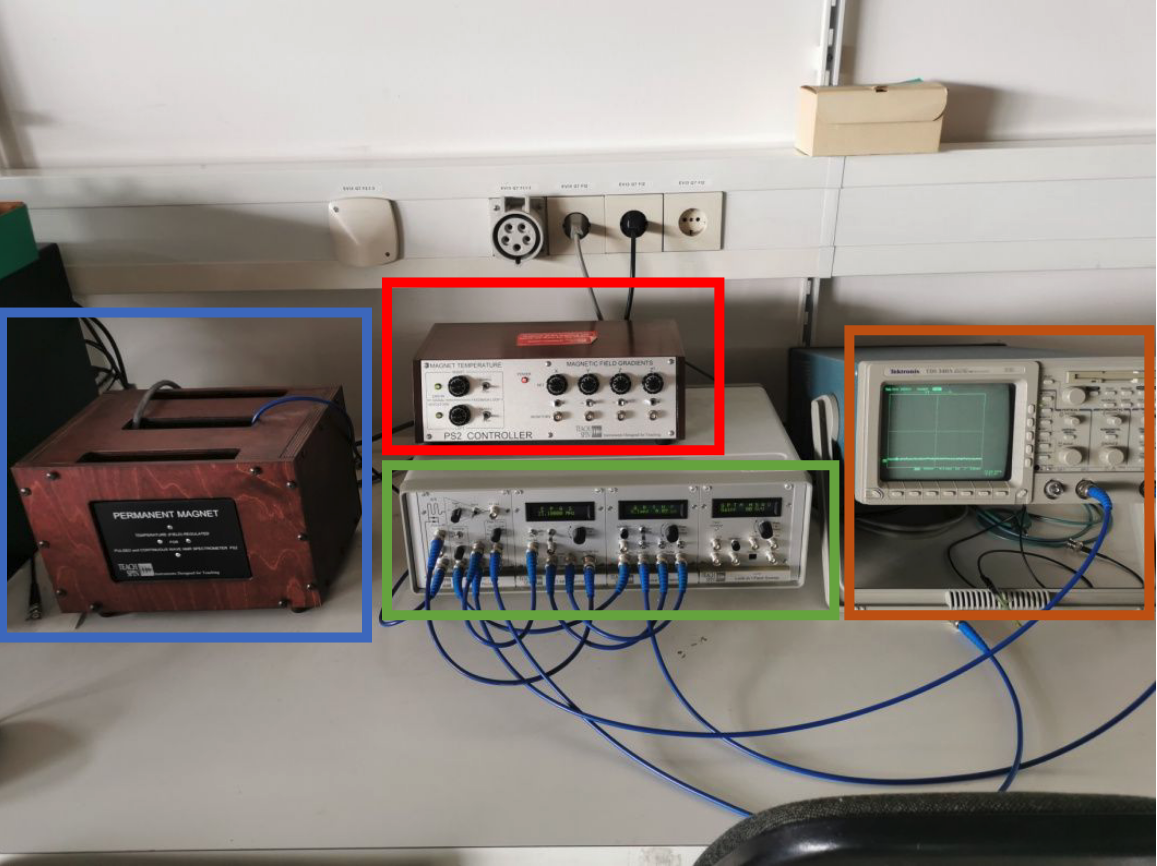
\includegraphics[width=0.7\textwidth]{exp_setup.png}
  \caption{
  blue box - permanent magnet \\
  red box - magnetic field gradients \\
  green box spectrometer console including rf synthesizer, pulse programmer and receiver unit \\ brown box oscilloscope.\cite{experimental_setup_manual}}
  \label{fig:example}
\end{figure}

\section{Experiment Procedure}

We will determine $T_1$ and $T_2$ for several concentrations of $CuSO_4$ and a light mineral oil by semi-logarithmic representation of the signal amplitudes over the time.

\begin{table}[h!]
\centering
\begin{tabular}{|c|c|c|c|c|}
\hline
 & \textbf{light mineral oil} & \textbf{.05 molar $CuSO_4$} & \textbf{.1 molar $CuSO_4$} & \textbf{.2 molar $CuSO_4$} \\ \hline
$T_1$ &&  &  & \\ \hline
$T_2$ &&  &  & \\ \hline
\end{tabular}
\caption{Values we will find experimentally}
\label{tab:example_table}
\end{table}

We begin by lookingg at the FID after applying a $90^o$ pulse, and do the following

\begin{itemize}
    \item \textbf{Pulse Length Adjustment} We maximize the signal intensity by adjusting the length of the applied pulse
    \item \textbf{Frequency Adjustment} until we've further maximized the intensity, and there are no off-resonance induced oscillations
    \item Adjust the shimming coils to minimize inhomogeneities
    \item record $T_2$ after doing all the above
    \item Optimize the $180^o$ pulse by varying $tau$ and other parameters. Here we want to maximize the echo and reduce the second pulse's FID
    \item Perform Car-Purcell experiment and the Meiboom-Gibson improvement
    \item Measure $T_1$ values by building a $180^o - \tau - 90^o$ sequence, varying $tau$, plotting the FID max, inverting the FID until the zero crossing, and doing an exponential fit.


\end{itemize}


% The reference list will be generated automatically based on the keys
% you use in your article and their metadata in the bibtex file
\bibliography{references}

\end{document}
